% Chapter X

\chapter{Determination of quark fragmentation functions into kaons} % Chapter title

\label{ch:FF} % For referencing the chapter elsewhere, use \autoref{ch:name}

%----------------------------------------------------------------------------------------

In the previous chapter, we obtained charged kaon multiplicities $M^K(x,Q^2,z)$. As these multiplicities can be expressed as a combination of the PDFs $q(x,Q^2)$ and the FFs $D^K_q(z,Q^2)$, assuming that the PDFs are known, we will use them to extract the quark fragmentation functions into kaon.

Two methods can be used to extract the multiplicities : a direct extraction and a fit. The direct extraction consists in extracting the FFs point by point. This method requires to have the same numbers of equation as the number of unknowns. The fit method is a simultaneous fit of all the data with predefined functional forms, including a $Q^2$ evolution in the fit.

The two methods are both relying on assumptions to decrease dramatically the number of FFs to determine.

\section{Direct extraction of quark fragmentation functions into kaons}

\subsection{Three fragmentation functions case}

Let us take the relation between the number of hadrons $\frac{dN^h}{dxdz}$, the unpolarized parton distributions $q(x,Q^2)$ and the fragmentation functions $D^h_q(z)$. By normalizing to the number of scattered leptons $\frac{dN^l}{dx}$, the relation gives at LO QCD :

\begin{equation} \label{eq:mult_basic}
  \frac{\frac{dN^h}{dxdQ^2dz}}{\frac{dN^l}{dxdQ^2}} = M^h(x,Q^2,z) = \frac{\sum_{q}e^2_qq(x,Q^2)\D{h}{q}(z))}{\sum_{q}e^2_q(x)}
\end{equation}

where $M^h(x,Q^2,z)$ is the multiplicities defined as in the SIDIS analysis \cite{Multiplicities}.
The sums are running over q = $u,d,s,\ubar,\dbar,\sbar$.

Explicitating the result for respectively proton Eq.\eqref{eq:mult_prot} and deuteron target Eq.\eqref{eq:mult_deut} \cite{Jorg}:

\begin{equation} \label{eq:mult_prot}
  M^h_p = \frac{4u\D{h}{u}+d\D{h}{d}+s\D{h}{s}+4\ubar\D{h}{\ubar}+\dbar\D{h}{\dbar}+\sbar\D{h}{\sbar}}{4(u+\ubar)+(d+\dbar)+(s+\sbar)}
\end{equation}

\begin{equation} \label{eq:mult_deut}
  M^h_d = \frac{(u+d)(4\D{h}{u}+\D{h}{d})+(\ubar+\dbar)(4\D{h}{\ubar}+\D{h}{\dbar})+2s\D{h}{s}+2\sbar\D{h}{\sbar}}{5(u+\ubar+d+\dbar)+2(s+\sbar)}
\end{equation}

Let us fix $h$ = $K^\pm$. In total there are 12 fragmentation functions arising from the expressions of $M^{K^+}$ and $M^{K^-}$. By assuming charge conjugation symmetry ($\D{K^+}{u}$ = $\D{K^-}{\ubar}$, etc.), this number is reduced to 6. These 6 fragmentation functions can then be classified in three groups (e.g. for $K^+$) : the favoured strange quark fragmentation function $\D{K^+}{str} = \D{K^+}{\sbar}$, the favoured up quark fragmentation function $\D{K^+}{fav} = \D{K^+}{u}$ and the unfavoured fragmentation functions $\D{K^+}{unf} = \D{K^+}{s},\D{K^+}{\ubar},\D{K^+}{\dbar},\D{K^+}{d}$, when assuming $\D{K^+}{s} = \D{K^+}{\ubar}$. This leads to the following equations :

\begin{equation} \label{eq:mult_prot_K+}
  M^{K^+}_p = \frac{4u\D{K}{fav}+\sbar\D{K}{str}+(4\ubar+s+d+\dbar)\D{K}{unf}}{4(u+\ubar)+(d+\dbar)+(s+\sbar)}
\end{equation}

\begin{equation} \label{eq:mult_prot_K-}
  M^{K^-}_p = \frac{4\ubar\D{K}{fav}+s\D{K}{str}+(4u+\sbar+d+\dbar)\D{K}{unf}}{4(u+\ubar)+(d+\dbar)+(s+\sbar)}
\end{equation}

\begin{equation} \label{eq:mult_deut_K+}
  M^{K^+}_d = \frac{4(u+d)\D{K}{fav}+2\sbar\D{K}{str}+((u+d)+5(\ubar+\dbar)+2s)\D{K}{unf}}{5(u+\ubar+d+\dbar)+2(s+\sbar)}
\end{equation}

\begin{equation} \label{eq:mult_deut_K-}
  M^{K^-}_d = \frac{4(\ubar+\dbar)\D{K}{fav}+2s\D{K}{str}+((\ubar+\dbar)+5(u+d)+2\sbar)\D{K}{unf}}{5(u+\ubar+d+\dbar)+2(s+\sbar)}
\end{equation}

As we only need three equations to have a Cramer system, we can combine Eq.\eqref{eq:mult_deut_K+} and Eq.\eqref{eq:mult_deut_K-} :

\begin{equation} \label{eq:mult_deut_K}
  M^{K}_d = \frac{4(u+d+\ubar+\dbar)\D{K}{fav}+2(s+\sbar)\D{K}{str}+(6(u+d+\ubar+\dbar)+2(s+\sbar))\D{K}{unf}}{5(u+\ubar+d+\dbar)+2(s+\sbar)}
\end{equation}

Eventually, the following system is obtained :

\begin{equation} \label{eq:mult_sys}
  \begin{split}
  \begin{pmatrix}
    M^{K^+}_p \\
    M^{K^-}_p \\
    M^{K}_d
  \end{pmatrix}
  = \\
  \begin{pmatrix}
    \frac{4u}{4(u+\ubar)+(d+\dbar)+(s+\sbar)} & \frac{\sbar}{4(u+\ubar)+(d+\dbar)+(s+\sbar)} & \frac{4\ubar+s+d+\dbar}{4(u+\ubar)+(d+\dbar)+(s+\sbar)} \\
    \frac{4\ubar}{4(u+\ubar)+(d+\dbar)+(s+\sbar)} & \frac{s}{4(u+\ubar)+(d+\dbar)+(s+\sbar)} & \frac{4u+\sbar+d+\dbar}{4(u+\ubar)+(d+\dbar)+(s+\sbar)} \\
    \frac{4(u+d+\ubar+\dbar)}{5(u+\ubar+d+\dbar)+2(s+\sbar)} & \frac{2(s+\sbar)}{5(u+\ubar+d+\dbar)+2(s+\sbar)} & \frac{6(u+d+\ubar+\dbar)+2(s+\sbar)}{5(u+\ubar+d+\dbar)+2(s+\sbar)}
  \end{pmatrix}
  \begin{pmatrix}
    \D{K}{fav} \\
    \D{K}{str} \\
    \D{K}{unf}
  \end{pmatrix}
  \end{split}
\end{equation}

Let us take a simple model where the nucleon is described by a valence ($q_v$) and a sea quark ($\qbar$) distribution, the quark distribution can be written as \cite{Jorg} :

\begin{center}
  \begin{tabular}{ l }
    $u = 2q_v + \alpha_u\qbar$ \\
    $d = q_v + \alpha_d\qbar$ \\
    $q = \alpha_q\qbar$ for $q=\ubar,\dbar,s,\sbar$ \\
  \end{tabular}
\end{center}

With this model, the previous matrix has the following form :

\begin{equation} \label{eq:mat_rank}
  \begin{pmatrix}
    \frac{8q_v+4\qbar}{9q_v+12\qbar} & \frac{\qbar}{9q_v+12\qbar} & \frac{q_v+7\qbar}{9q_v+12\qbar} \\
    \frac{4\qbar}{9q_v+12\qbar} & \frac{\qbar}{9q_v+12\qbar} & \frac{9q_v+7\qbar}{9q_v+12\qbar} \\
    \frac{12q_v+16\qbar}{15q_v+24\qbar} & \frac{4\qbar}{15q_v+24\qbar} & \frac{18q_v+28\qbar}{15q_v+24\qbar}
  \end{pmatrix}
\end{equation}

Assuming that the PDFs are not pathological, one is assured that the rank of this matrix is 3, then the extraction is feasible.

By performing a matrix inversion, the result of $\D{K}{fav}(z)$, $\D{K}{str}(z)$ and $\D{K}{unf}(z)$ can be obtained using data from various $(x,y)$ bins which in fact cover different $Q^2$ ranges.

\subsection{Extension to four fragmentation functions into kaons}

As there were initially 4 fragmentation functions, we can adress the question of the assumption
$\D{K^+}{s}=\D{K^+}{\ubar}=\D{K^+}{\dbar}=\D{K^+}{d}$ used in the previous section (3 independent kaon FFs). From PYTHIA simulation, one can find the following
values for the fragmentation functions :

\begin{center}
  \begin{tabular}{ || c | c | c || }
    \hline \hline
    quark $q$ & hadron $h$ & $\int_{0.2}^{1}\D{h}{q}dz$ \\ \hline
    $\sbar$ & $K^+$ & 0.35 \\
    $u$ & $K^+$ & 0.09 \\
    $d$ & $K^+$ & 0.06 \\
    $s$ & $K^+$ & 0.05 \\
    $\ubar$ & $K^+$ & 0.03 \\
    $\dbar$ & $K^+$ & 0.03 \\
    \hline \hline
  \end{tabular}
\end{center}

The table clearly points that for example, $\D{K^+}{d} \approx 2\D{K^+}{\dbar}$. This can be explained
in this case from the fact that $K^+$ may originate from $K^{0*} = (d\sbar) \rightarrow K^+\pi^+$ and
not from $\bar{K}^{0*} \rightarrow K^-\pi^+$.

A new unfavoured fragmentation function can be added by splitting the former unfavoured one into two, viz. :

\begin{center}
  \begin{tabular}{ l }
    $\D{K}{fav}=\D{K^+}{u}$ \\
    $\D{K}{str}=\D{K^+}{\sbar}$ \\
    $\D{K}{unf_1}=\D{K^+}{s}=\D{K^+}{d}$ \\
    $\D{K}{unf_2}=\D{K^+}{\ubar}=\D{K^+}{\dbar}$ \\
  \end{tabular}
\end{center}

Thus, the system is :

\begin{equation} \label{eq:mult_sys4}
  \begin{split}
  \begin{pmatrix}
    M^{K^+}_p \\
    M^{K^-}_p \\
    M^{K^+}_d \\
    M^{K^-}_d \\
  \end{pmatrix}
  = \\
  \begin{pmatrix}
    \frac{4u}{4(u+\ubar)+(d+\dbar)+(s+\sbar)} & \frac{\sbar}{4(u+\ubar)+(d+\dbar)+(s+\sbar)} & \frac{s+d}{4(u+\ubar)+(d+\dbar)+(s+\sbar)} & \frac{4\ubar+\dbar}{4(u+\ubar)+(d+\dbar)+(s+\sbar)} \\
    \frac{4\ubar}{4(u+\ubar)+(d+\dbar)+(s+\sbar)} & \frac{s}{4(u+\ubar)+(d+\dbar)+(s+\sbar)} & \frac{\sbar+\dbar}{4(u+\ubar)+(d+\dbar)+(s+\sbar)} & \frac{4u+d}{4(u+\ubar)+(d+\dbar)+(s+\sbar)} \\
    \frac{4(u+d)}{5(u+\ubar+d+\dbar)+2(s+\sbar)} & \frac{2\sbar}{5(u+\ubar+d+\dbar)+2(s+\sbar)} & \frac{u+d+2s}{5(u+\ubar+d+\dbar)+2(s+\sbar)} & \frac{5(\ubar+\dbar)}{5(u+\ubar+d+\dbar)+2(s+\sbar)} \\
    \frac{4(\ubar+\dbar)}{5(u+\ubar+d+\dbar)+2(s+\sbar)} & \frac{2s}{5(u+\ubar+d+\dbar)+2(s+\sbar)} & \frac{\ubar+\dbar+2\sbar}{5(u+\ubar+d+\dbar)+2(s+\sbar)} & \frac{5(u+d)}{5(u+\ubar+d+\dbar)+2(s+\sbar)}
  \end{pmatrix}
  \begin{pmatrix}
    \D{K}{fav} \\
    \D{K}{str} \\
    \D{K}{unf_1} \\
    \D{K}{unf_2}
  \end{pmatrix}
\end{split}
\end{equation}

Let us take again the same simple model for quark distributions, with $q_v$ (valence) and $\bar{q}$ (sea) quark distributions, leading to the following matrix :

\begin{equation} \label{eq:mat_rank_4E}
  \begin{pmatrix}
    \frac{8q_v+4\qbar}{9q_v+12\qbar} & \frac{\qbar}{9q_v+12\qbar} & \frac{q_v+2\qbar}{9q_v+12\qbar} & \frac{5\qbar}{9q_v+12\qbar} \\
    \frac{4\qbar}{9q_v+12\qbar} & \frac{\qbar}{9q_v+12\qbar} & \frac{2\qbar}{9q_v+12\qbar} & \frac{9q_v+5\qbar}{9q_v+12\qbar} \\
    \frac{12q_v+8\qbar}{15q_v+24\qbar} & \frac{2\qbar}{15q_v+24\qbar} & \frac{3q_v+4\qbar}{15q_v+24\qbar} & \frac{10\qbar}{15q_v+24\qbar} \\
    \frac{8\qbar}{15q_v+24\qbar} & \frac{2\qbar}{15q_v+24\qbar} & \frac{4\qbar}{15q_v+24\qbar} & \frac{15q_v+10\qbar}{15q_v+24\qbar}
  \end{pmatrix}
\end{equation}

Assuming that the PDFs are not pathological, one is assured that the rank of this matrix is 4, then the extraction
is feasible.

\subsection{Application to extracted kaon multiplicities}

The two methods were tested to extract the FFs directecly from the kaon multiplicities. Unfortunately, it appears that the methods are not working as expected. The hypothesis that the formulas linking multiplicities to PDFs and FFs for a proton and a deuteron target should be enough decoupled to do a combined extraction of the FFs is not right. The only way to extract the FFs into kaons from the kaon multiplicities is then the LO QCD fit of multiplicities.

%----------------------------------------------------------------------------------------

\section{Extraction of quark fragmentation functions into kaons from a LO QCD fit of kaon multiplicities}

The extraction of FFs from the measured $K^{\pm}$ multiplicities is performed in a LO pQCD fashion according to Eq. \ref{eq:MultpQCD} :

\begin{equation}
  \frac{dM^h(x,Q^2,z)}{dz} = \frac{d^3\sigma^h(x,Q^2,z)/dxdQ^2dz}{d^3\sigma^{DIS}(x,Q^2,z)/dxdQ^2} = \frac{\sum_q e^2_q(x,Q^2)D^h_q(z,Q^2)}{\sum_q e^2_qq(x,Q^2)}
\end{equation}

with $q(x,Q^2)$ are the quark PDFs for the flavour $q$. Using a standard $\chi^2$ minimization over the data points :

\begin{equation} \label{eq:MultpQCD}
  \chi^2 = \sum_j \frac{\left[T_j\left(x_j,Q^2_j,z_j\right) - M_j\left(x_j,Q^2_j,z_j\right)\right]^2}{\sigma^2_j}
\end{equation}

where $M_j$ are the measured multiplicities and $\sigma^2_j$ are the quadratic sum of the statistical and systematic errors. $T_j$ are the multiplicities evaluated for a set of parameters for a given parametrisation. Due to the large $Q^2$ span covered by the data, it is mandatory to properly take into account the $Q^2$ dependence of FFs and PDFs. Thus the $T_j$ are evaluated at $Q^2_0$ = 1 (GeV/$c$)$^2$ and evolved to tehir actual $Q^2_j$ using a DGLAP $Q^2$ evolution code provided by M. Hirai and S. Kumano \cite{}.

For the combined analysis of $K^+$ and $K^-$ multiplicities, isospin and charge symmetry are imposed. This yields to four independent FFs :

\begin{center}
  \begin{tabular}{ l }
    $\D{K}{fav}=\D{K^{\pm}}{fav}=\D{K^+}{u}=\D{K^-}{\ubar}$ \\
    $\D{K}{s}=\D{K^{\pm}}{s}=\D{K^+}{\sbar}=\D{K^-}{s}$ \\
    $\D{K}{unf}=\D{K^{\pm}}{unf}=\D{K^+}{\ubar}=\D{K^-}{u}=\D{K^+}{s}=\D{K^-}{\sbar}=\D{K^{\pm}}{d}=\D{K^{\pm}}{\dbar}$ \\
    $\D{K}{glu}=\D{K^{\pm}}{glu}$ \\
  \end{tabular}
\end{center}

For the current analysis, the following parametrization is used :

\begin{equation}
  \begin{split}
    zD_i(z,Q^2_0) = \frac{N_i z^{\alpha_i} (1-z)^{\beta_i} (1+\gamma_i(1-z)^{\delta_i})}{\int_{0.2}^{0.85} z'^{\alpha_i} (1-z')^{\beta_i} (1+\gamma_i(1-z')^{\delta_i} dz'},\,i=\{fav\} \\
    zD_i(z,Q^2_0) = \frac{N_i z^{\alpha_i} (1-z)^{\beta_i}}{\int_{0.2}^{0.85} z'^{\alpha_i} (1-z')^{\beta_i} dz'},\,i=\{s,unf,g\}
  \end{split}
\end{equation}

The PDFs set from MSTW08 in LO \cite{}, provided by the LHAPDF data group \cite{} was chosen. The fits of the data for $K^+$ and $K^-$ are shown in Fig. \ref{pic:MFitK}.

\begin{figure}[!h]
  \centering
	% \subfloat[$K^+$]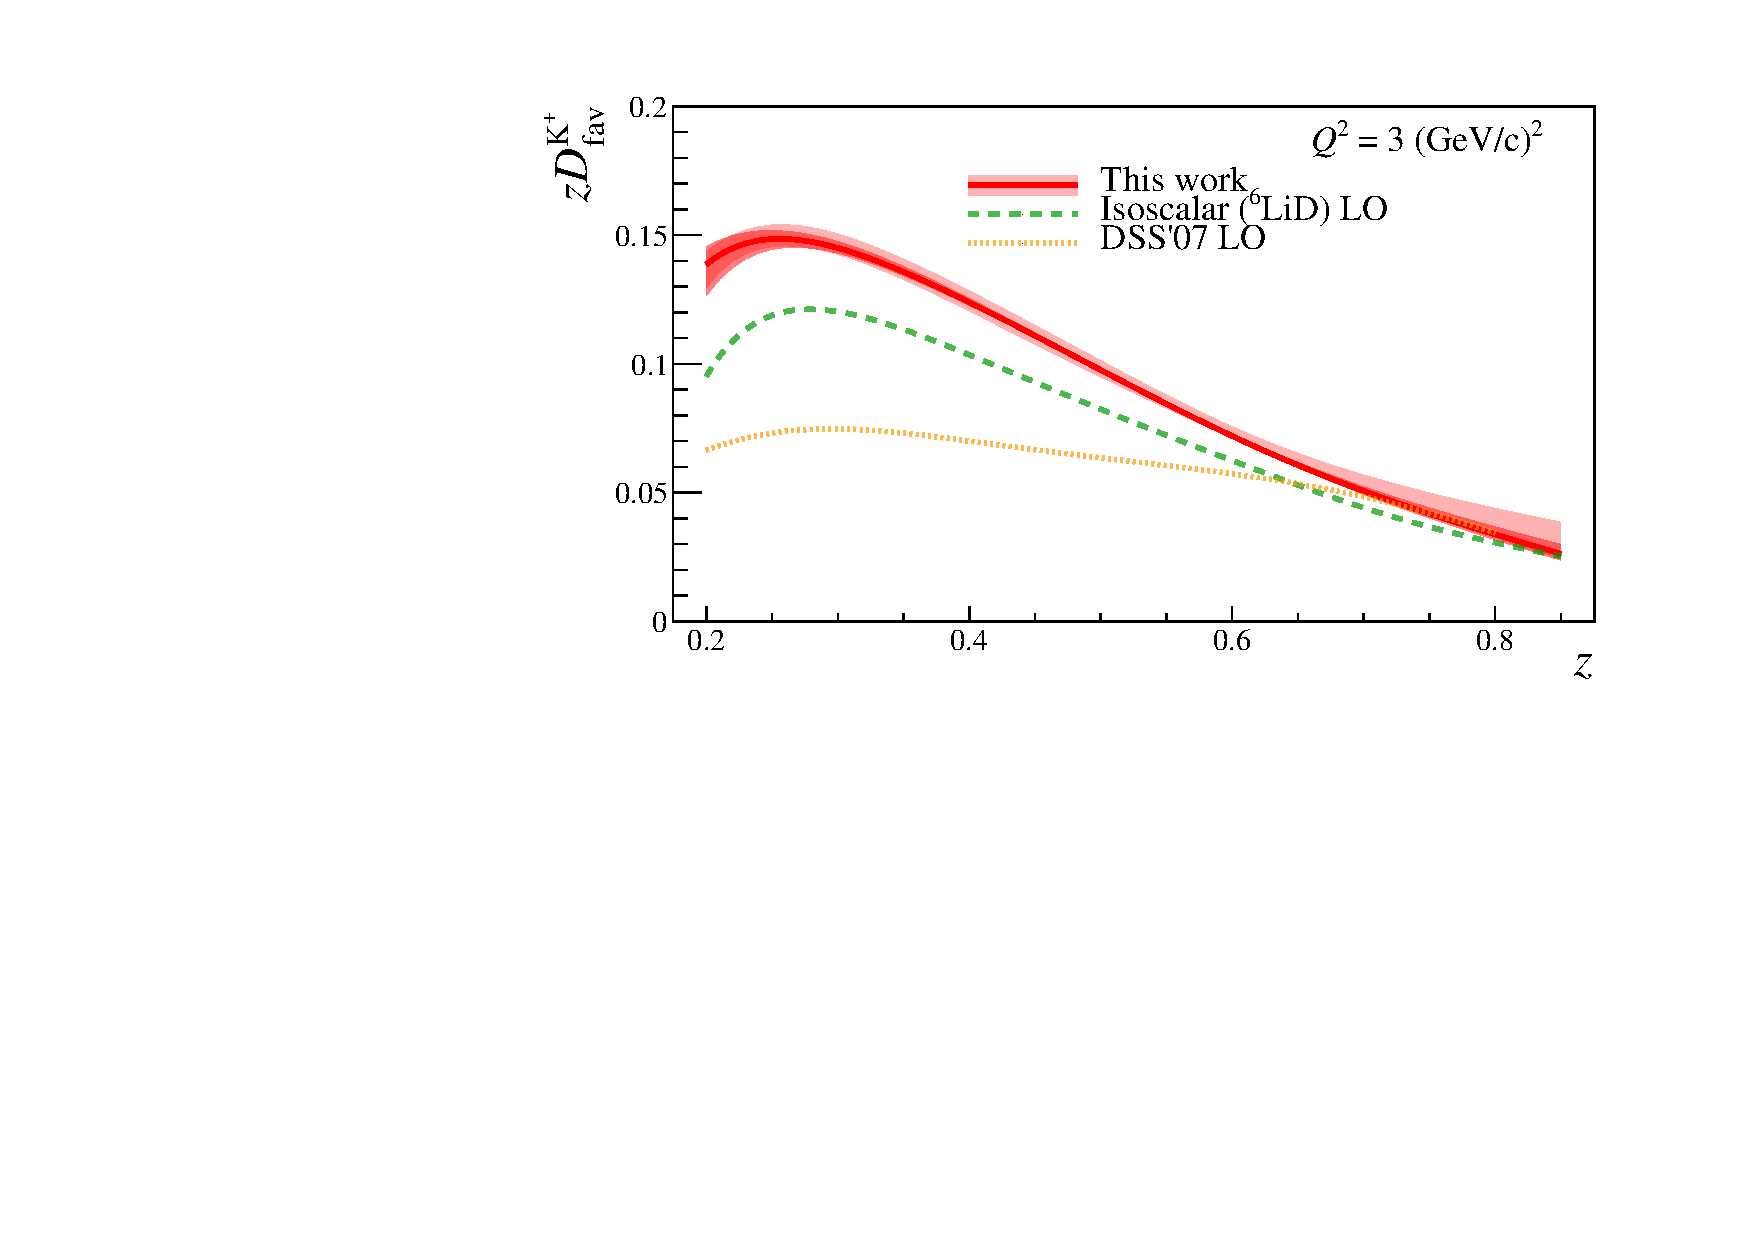
\includegraphics[scale=0.4]{./gfx/fav.pdf}
  % \subfloat[$K^-$]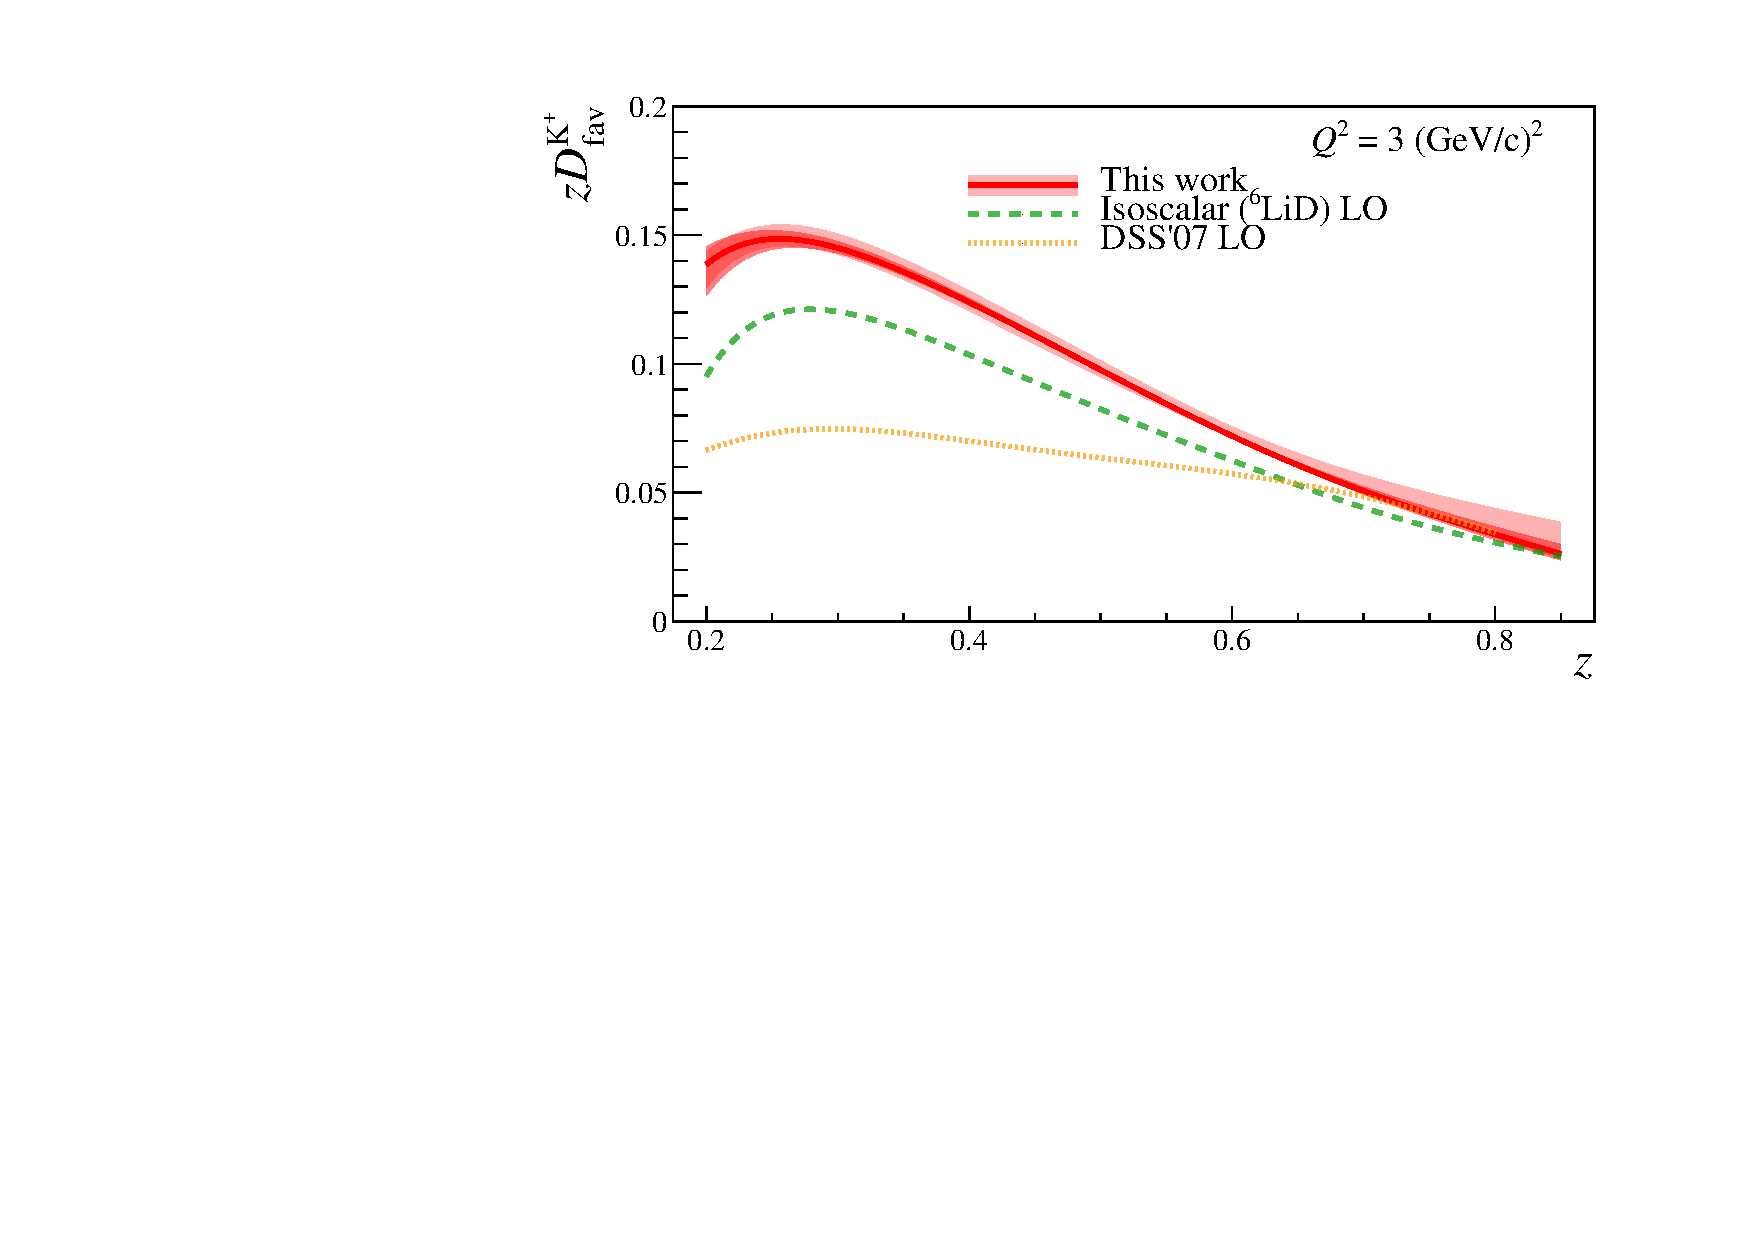
\includegraphics[scale=0.4]{./gfx/fav.pdf}
  \caption{$K^+$ (a) and $K^-$ (b) multiplicities versus $z$ in bins of $z$ and scattered vertically with $y$. The curves correspond to the LO fit of $K^{\pm}$ multiplicities.}
	\label{pic:MFitK}
\end{figure}


To determine the uncertainties of the extracted FFs, the replica method \cite{} is used. A number of resamples of the original multiplicity dataset is constructed. A reample is constructed by adding noise randomly generated from a zero-centered gaussian with a width of the data point's error to each data point of the oiginal dataset. Then, for each resample the FFs are extracted using the same fit procedure than for the real dataset. The error is then determined as the mean value with RMS of the extracted FFs from the resamples. For the current analysis, 100 replicas are used. Error bands for statistical and systematic errors are calculated. As it is assumed that the systematic errors are correlated, each resample's systematic error is weighted by the same randomly determined value. For both statistical and systematic error bands, the statistical errors are used for the calculation of the $\chi^2$.

The final parameters of the fit are displayed in Table. \ref{tab:Fitparam}. The $\chi^2$ per degrees of freedom for the results is of 3.5. In Fig. \ref{pic:FFFit}, the four FFs are shown. The values obtained are significantly higher for $\D{K}{fav}$ and $\D{K}{unf}$ compared to DSEHS results.

\begin{table}[!h]
  \begin{center}
    \begin{tabular}{ | c | c c c c c | }
      \hline
      \hline
       & N & $\alpha$ & $\beta$ & $\gamma$ & $\delta$ \\
      \hline
      \hline
      $\D{K}{fav}$ & 0.0647 $\pm$ 0.0007 & -1.2 $\pm$ 0.2 & 0.46 $\pm$ 0.07 & -1.6 $\pm$ 0.7 & 3.4 $\pm$ 0.2 \\
      $\D{K}{s}$ & 0.03 $\pm$ 0.01 & 14 $\pm$ 7 & 27 $\pm$ 10 & - & -  \\
      $\D{K}{unf}$ & 0.005 $\pm$ 2 & 4 $\pm$ 5 & 19 $\pm$ 10 & - & - \\
      $\D{K}{glu}$ & 0.08 $\pm$ 0.1 & 16 (fixed) & 11 (fixed) & - & - \\
      \hline
      \hline
    \end{tabular}
  \end{center}
  \caption{Fit parameters for $Q^2_0$ = 1 (GeV/$c$)$^2$. The associated $\chi^2$ is of 3.5.}
  \label{tab:Fitparam}
\end{table}


\begin{figure}[!h]
  \centering
	\subfloat[$zD^{K}_{fav}$]{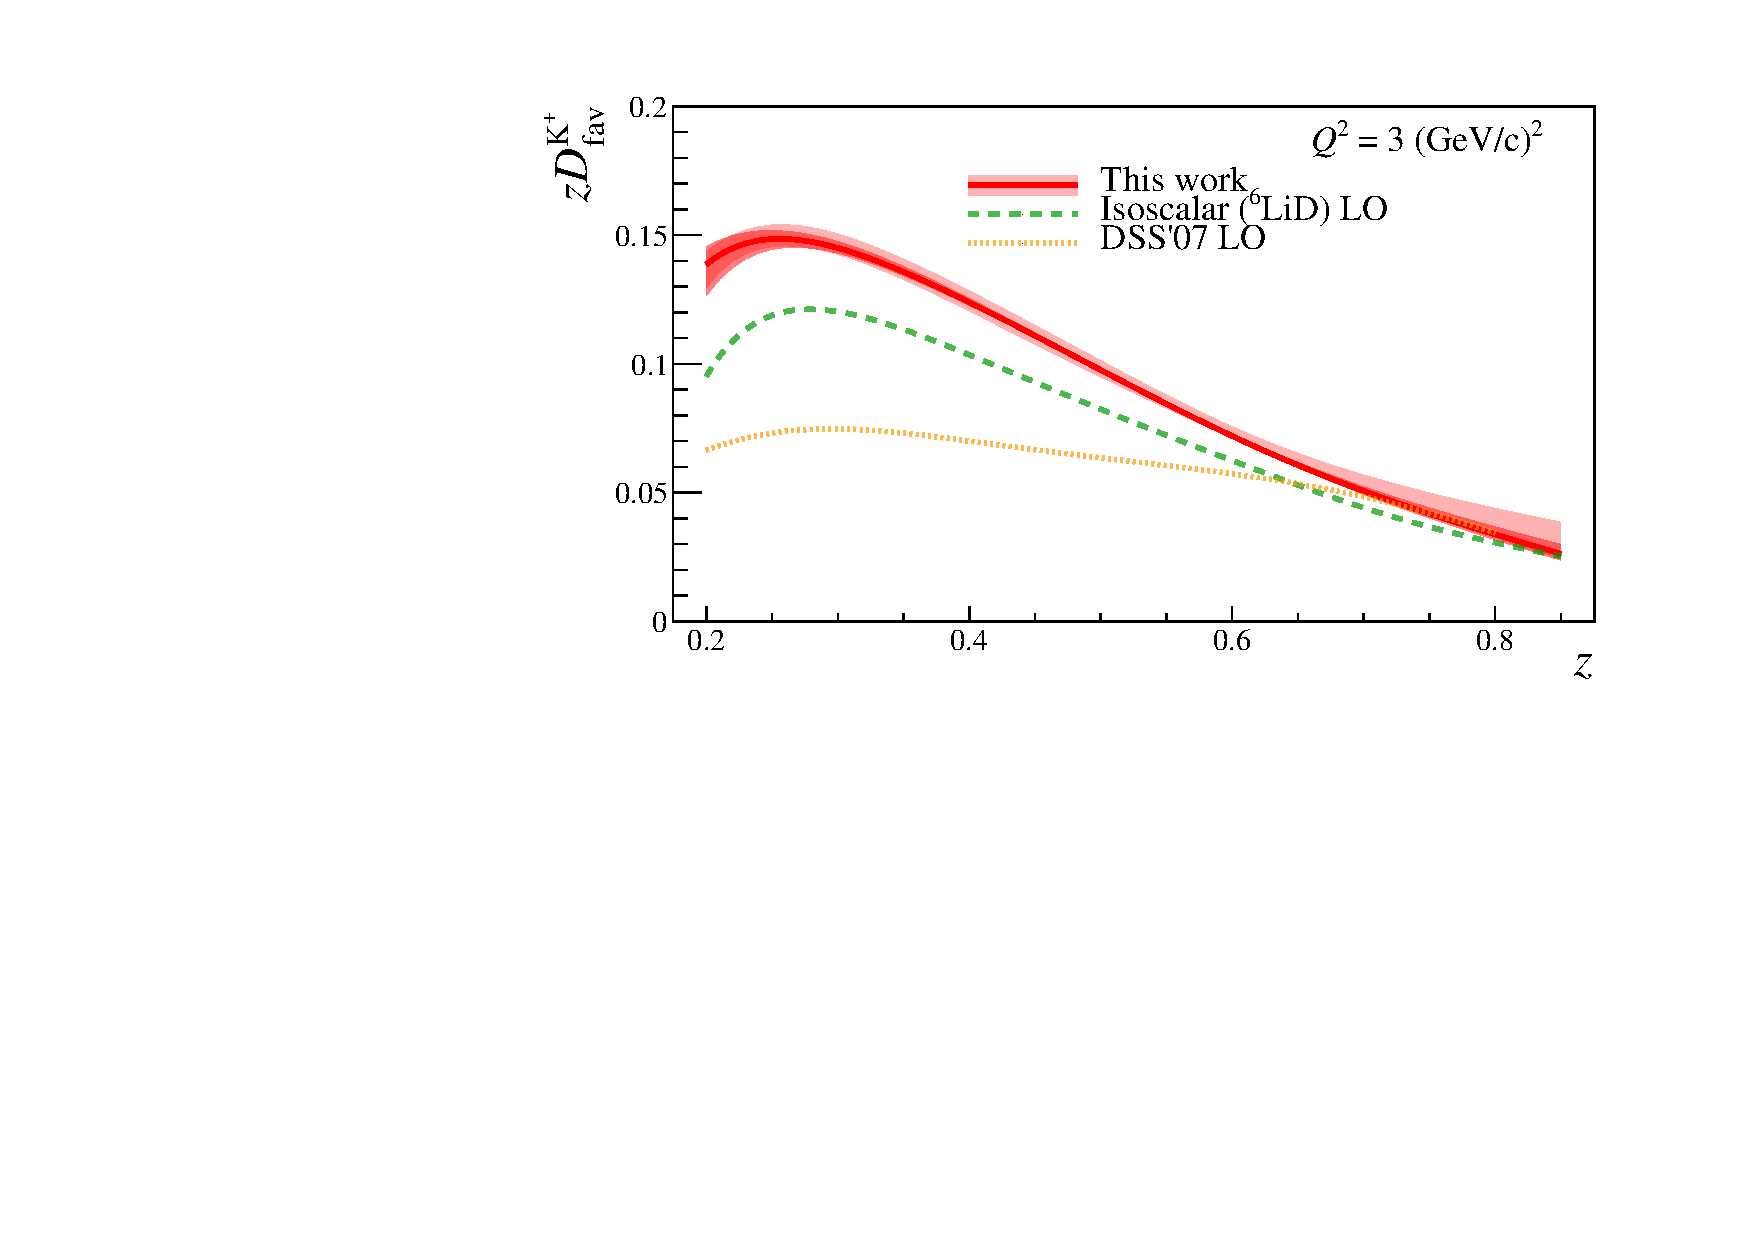
\includegraphics[scale=0.4]{./gfx/fav.pdf}}
  \subfloat[$zD^{K}_{unf}$]{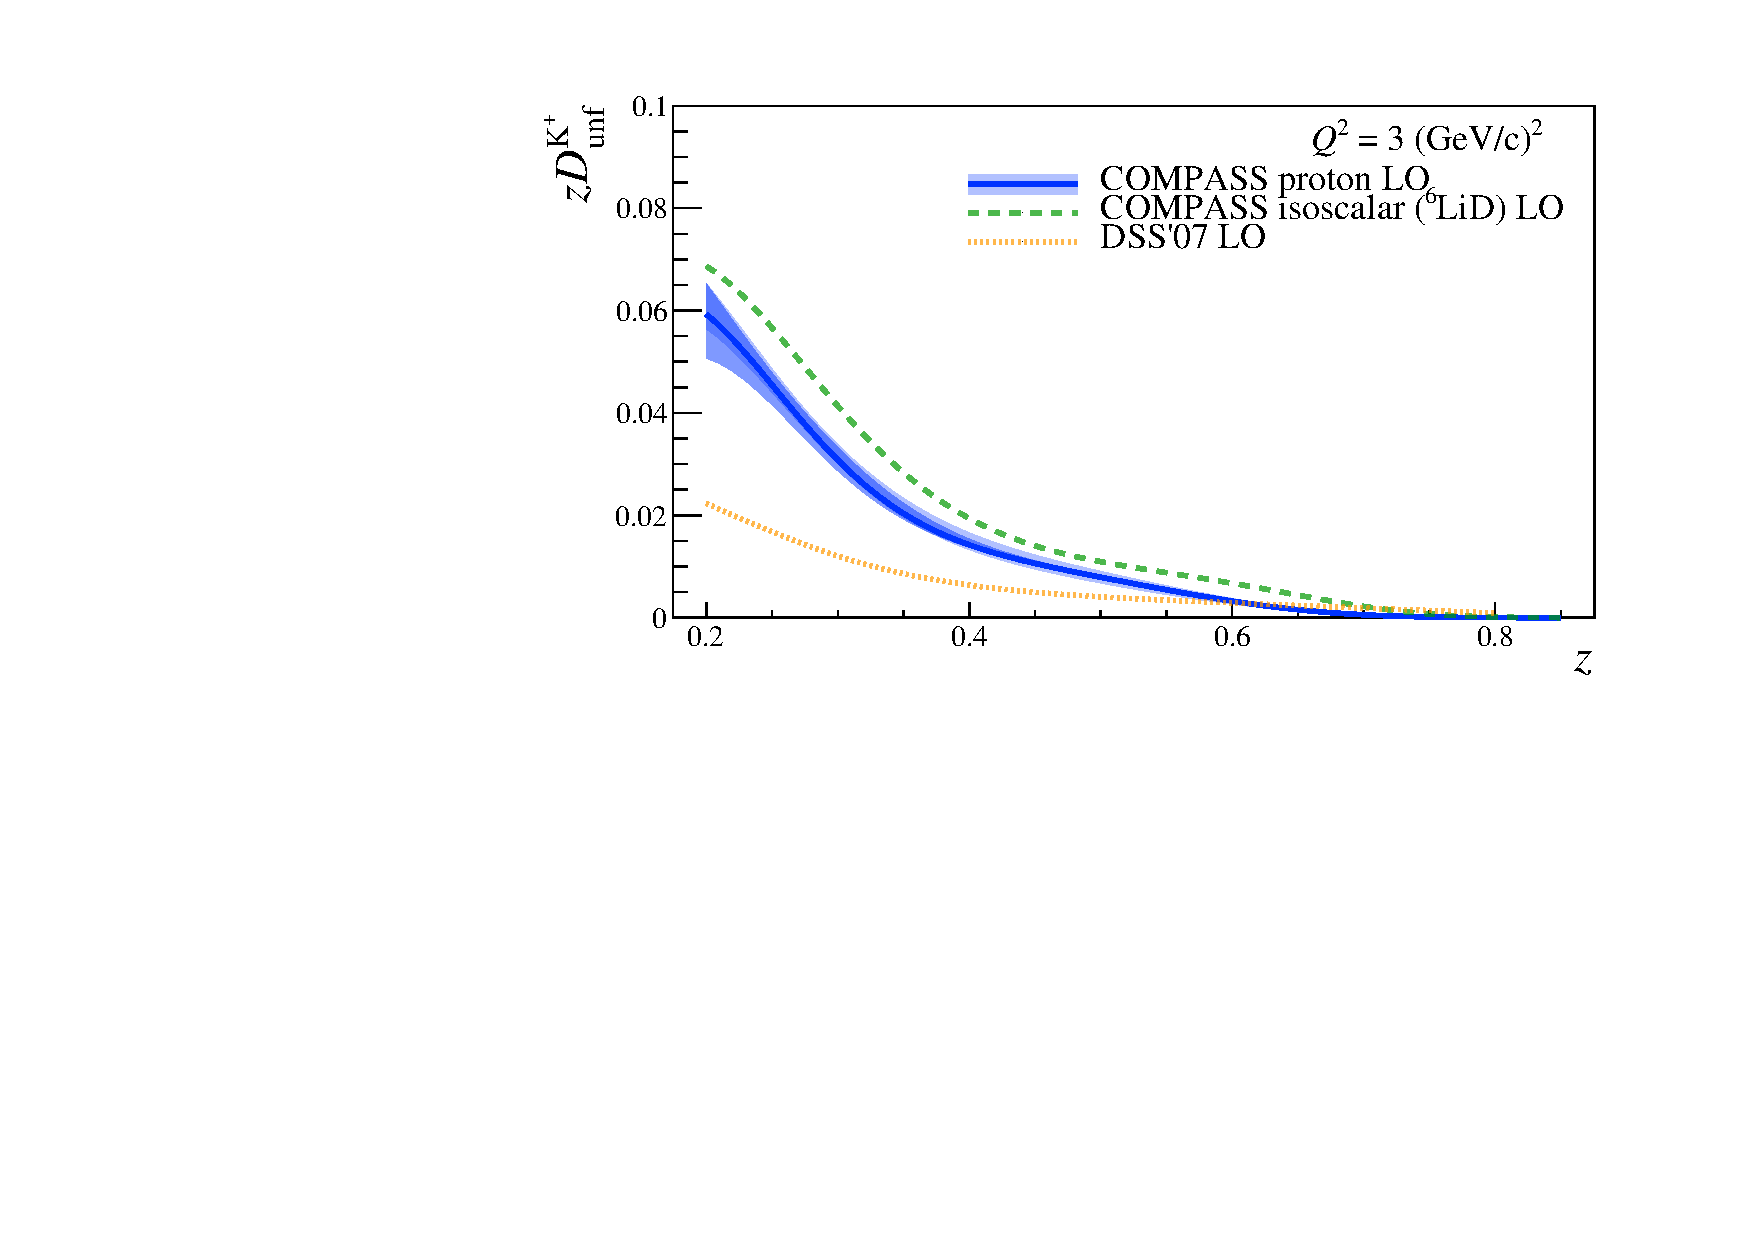
\includegraphics[scale=0.4]{./gfx/unf.pdf}} \\
  \subfloat[$zD^{K}_{s}$]{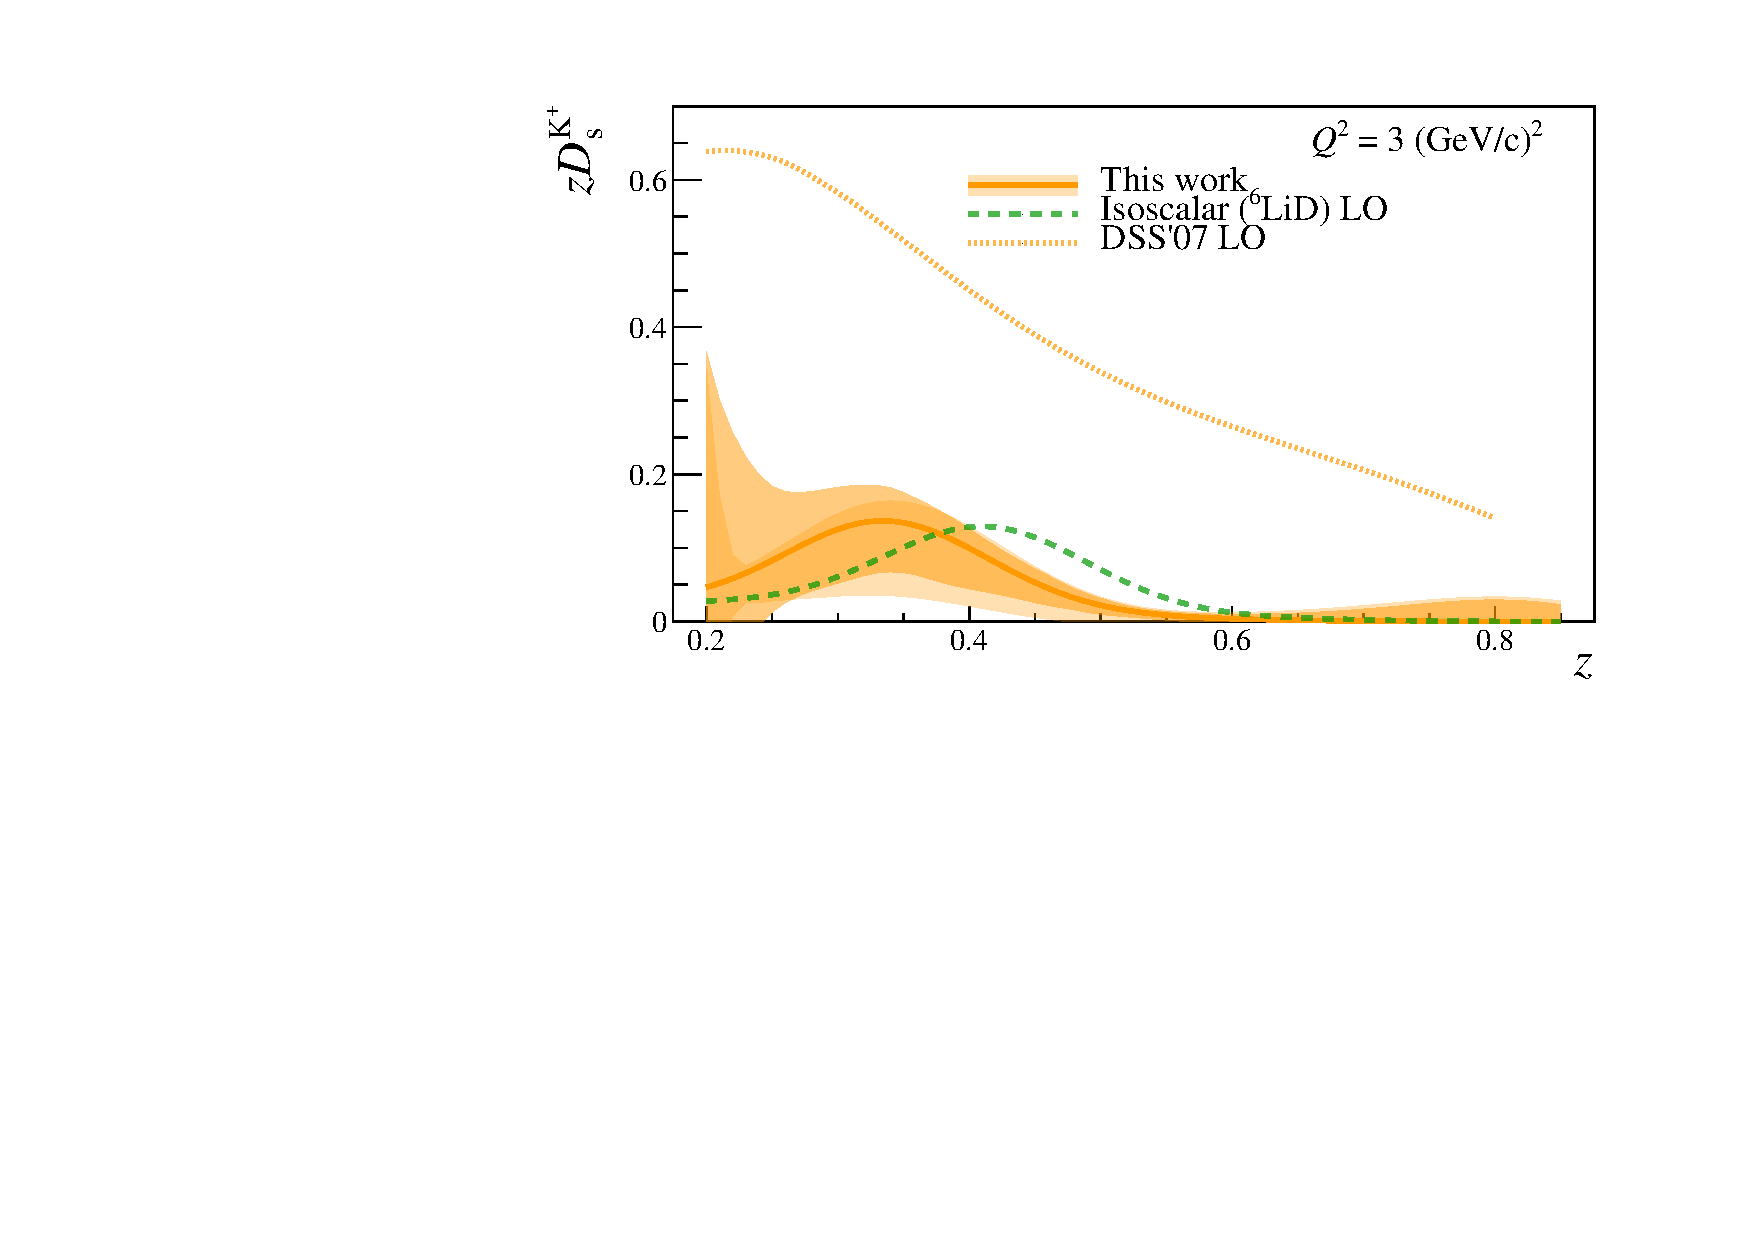
\includegraphics[scale=0.4]{./gfx/sbar.pdf}}
  \subfloat[$zD^{K}_{g}$]{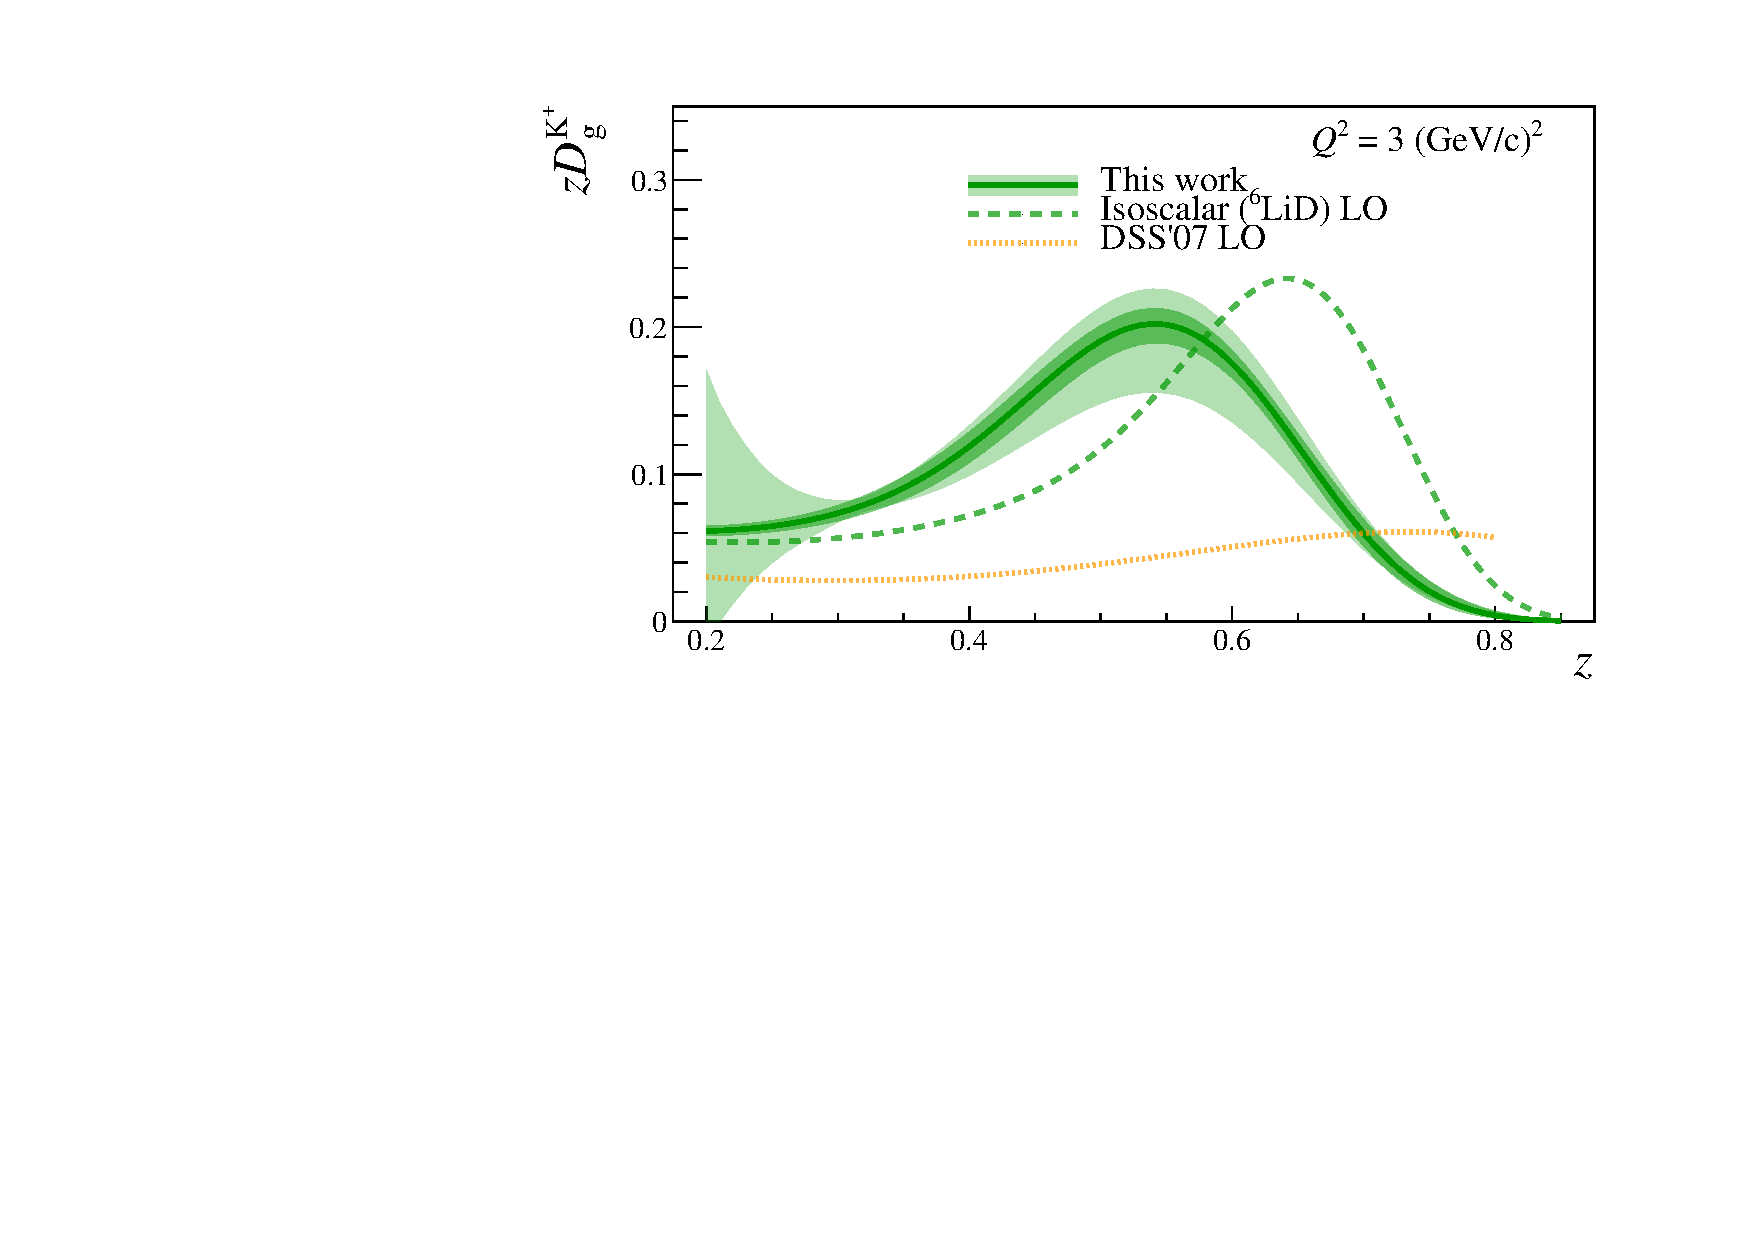
\includegraphics[scale=0.4]{./gfx/gluon.pdf}}
	\caption{The favoured (top left), unfavoured (top right), strange (bottom left) and gluon (bottom right) quark FFs $zD(z)$ into kaons from the COMPASS LO fit. The fit is done based on both the statistical and systematic errors.}
	\label{pic:FFFit}
\end{figure}

%----------------------------------------------------------------------------------------

\newpage

\section{Summary}

Kaon fragmentation functions have been extracted from a fit at LO of the charged kaon multiplicities. They have been extracted in the 0.2-0.85 $z$ domain. The direct extraction was considered due to the fact that multiplicities for a proton target and an isoscalar target have different equation linking them to PDFs and FFs. Nevertheless, the multiplicities for proton and isoscalar targets are still too similar to do such an extraction. Though the fit is still not stable due to the preliminary character of the multiplicities, it shows that the results from fragmentation functions are not far from what was obtained from COMPASS for an isoscalar target. (+ comparison with DSEHS and JAM)

These data represent a high statistics data set which will be helpful for NLO QCD fits of world data. They will constrain the values of quark FFs into kaons at moderate $Q^2$.
